\chapter{Inference Tasks}\label{chap:in_inference_tasks} % (fold)
For \textbf{models} with hidden/classification values inferring them, given a value in the data space:
\begin{itemize}
    \item for \hyperref[def:pcfg]{PCFG} model, parsing a sentence, considering all possible ways of generating a sentence, to \textbf{infer} its most probable \hyperref[def:pg-syntax-tree]{Syntax Tree};
    \item for \hyperref[sub:lm_mixture_of_bag_of_words]{Mixture of Bag-of-Words} model classifying a sentence, considering all possible ways of generating a given sentence to \textbf{infer} its most probable category;
    \item for \hyperref[def:hmm]{Hidden Markov Model}, considering all possible ways of generating a sequence of observations to \textbf{infer} its most probable sequence of categories;
\end{itemize}
We distinguish:
\begin{itemize}
    \item \textbf{\ac{map}} inference task: infers the \textbf{most probable hidden structure} given the observed string $w$;
    \item \textbf{Posterior probability distribution inference} task: infers the \textbf{probability distribution over all possible hidden structures} given the observed string $w$;
        \begin{note}
            It can also be \textbf{marginalized} to obtain a distribution over only some components of the hidden structures, e.g. filtering in \hyperref[def:hmm]{Hidden Markov Models} for distribution over the last state
        \end{note}
\end{itemize}
In general, \textbf{A Posterior Probability} is a probability over \textbf{hidden structures} once a specific observed string is given (\textbf{conditional probability}). 
\begin{note}[Technically]
    There is also a more basic inference task: \textbf{Observed String Probability} $P(w)$ inference task.
    It infers the total probability of generating, via all possible hidden structures,  the observed string $w$, also called \textbf{likelihood} of $w$ in the model
\end{note}
%
\section{PCFG Inference Task}\label{sec:in_pcfg_inference_task} % (fold)
\begin{example}{}{}
    Parsing of ``I can fish'' infers \hyperref[def:pg-syntax-tree]{Syntax Trees} $T_1$ and $T_2$
    \begin{cimage}
        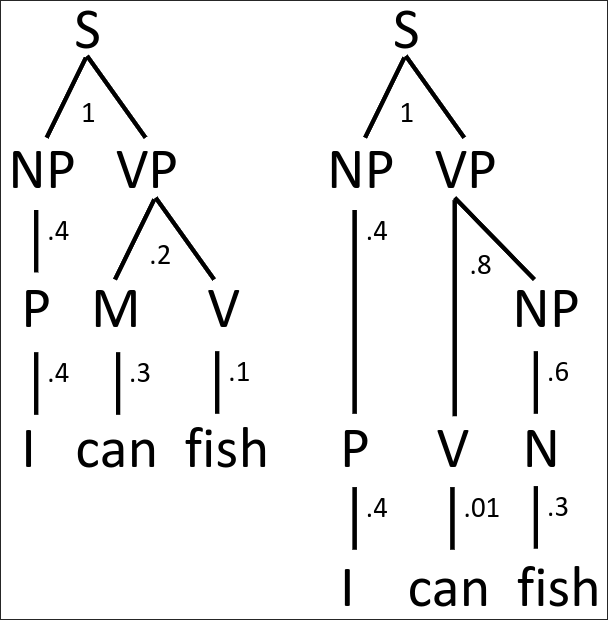
\includegraphics[width=.4\textwidth]{assets/20261119_123753.png}
    \end{cimage}
    \[
        \begin{aligned}
            S&\to NP\ VP[1.0] \\
            NP&\to Noun[0.6]\ |\ Pronoun[0.4] \\
            VP&\to Verb\ NP[0.8]\ |\ Modal\ Verb[0.2] \\
              &\\
            Noun&\to fish[0.3]\ |\ \dots \\
            Pronoun&\to I[0.4]\ |\ they[0.3]\ |\ \dots \\
            Verb&\to can[0.01]\ |\ fish[0.1]\ |\ \dots \\
            Modal&\to can[0.3]\ |\ \dots
        \end{aligned}
    \]
    \[
        \begin{aligned}
            &P(T_1) = 1\cdot0.4\cdot0.4\cdot0.2\cdot0.3\cdot0.1 = 0.00096 \\
            &P(T_2) = 1\cdot0.4\cdot0.4\cdot0.8\cdot0.01\cdot0.6\cdot0.3 = 0.0002304 \\
            &P_G(w) = P_G(T_1) + P_G(T_2) = 0.0011904
        \end{aligned}
    \]
    \end{example}
\begin{description}
    \item[Maximum A Posteriori] It infers the \hyperref[def:pg-syntax-tree]{Syntax Tree} generating $w$ that has \textbf{maximum probability}, formally:
        \[
            T' = \argmax_{T\in Tree_G(w)}P_G(T)
        \]
        In general, the number $|Tree_G(w)|$, the cardinality of $Tree_G(w)$, of \hyperref[def:pg-syntax-tree]{Syntax Trees} $T$ to consider, for finding such $T'$, is \textbf{exponential} in the length of $w$.
        \begin{note}
            Nevertheless, a \textbf{polynomial algorithm} exists: the \textbf{\ac{pcyk}} algorithm
        \end{note}
    \item[Posterior Probability Distribution] For any \hyperref[def:pg-syntax-tree]{Syntax Tree} generating $w$, it infers its \textbf{conditional probability}, given that $w$ is generated:
        \[
            \frac{P_G(T_1)}{P_G(w)},\,\frac{P_G(T_2)}{P_G(w)} \qquad \text{with: }P_G(w) = P_G(T_1) + P_G(T_2)
        \]
        Formally, it infers for any $T\in Tree_G(w)$:
        \[
            \ba[G]{T}{w} = \dfrac{\p[G]{T}}{\p[G]{w}}
        \]
        In general $P_G(w) = \sum_{T\in Tree_G(w)}{P_G(T)}$ is computed by the \textbf{observed string probability inference} task:
        \begin{itemize}
            \item number $|Tree_G(w)|$ of \hyperref[def:pg-syntax-tree]{Syntax Tree} $T$ to consider, is \textbf{exponential} in the length of $w$;
            \item nevertheless, a \textbf{polynomial algorithm} exists: the \textbf{Inside Algorithm}, a variant of \hyperref[sub:ll_algoritmo_cyk]{CYK};
        \end{itemize}
\end{description}
\begin{note}
    The \ac{map} inference task, correctly infers the \hyperref[def:pg-syntax-tree]{Syntax Tree}  $T'$ with maximum conditional probability:
    \[
        \ba[G]{T'}{w} = \frac{P_G(T')}{P_G(w)}
    \]
    in that:
    \[
        T' = \argmax_{T\in Tree_G(w)}P_G(T) = \argmax_{T\in Tree_G(w)}\frac{P_G(T)}{P_G(w)}
    \]
\end{note}
%
\subsection{Chomsky Normal Form for PCFGs}\label{sub:in_chomsky_normal_form_for_pcfgs} % (fold)
As for the \hyperref[sub:ll_algoritmo_cyk]{CYK} algorithm, its probabilistic versions \textbf{\ac{pcyk}} and \textbf{Inside} need the \hyperref[def:pcfg]{PCFG} to be in \hyperref[def:cnf]{CNF}:
\[
    \begin{aligned}
        A&\to BC[p],\text{ with } \pg{A,B,C}\subset V \\
        A&\to a[p],\text{ with } A\in V,\, a\in\Sigma
    \end{aligned}
\]
For each \hyperref[def:pcfg]{PCFG} $G$ such that $P_G(\epsilon) = 0$ there exists an \textbf{equivalent} \hyperref[def:pcfg]{PCFG} $G'$ in \hyperref[def:cnf]{CNF}.
% subsection Chomsky Normal Form for PCFGs (end)
%
\subsection{PCFG Inference Algorithm}\label{sub:in_pcfg_inference_algorithm} % (fold)
We use this \hyperref[def:pcfg]{PCFG} $G$ to exemplify \textbf{\ac{pcyk}} and \textbf{Inside} inference algorithms.
\emptyln{}
We start from the \textbf{\ac{pcyk}} algorithm that performs the \textbf{\ac{map}} inference task.
It efficiently infers the \hyperref[def:pg-syntax-tree]{Syntax Tree} generating $w$ that has \textbf{maximum probability}.
\[
    T' = \argmax_{T\in Tree_G(w)}{P_G(T)}
\]
\begin{note}
    Same computational complexity as \hyperref[sub:ll_algoritmo_cyk]{CYK}: $O(N^3)$ with $n = |w|$.
\end{note}
%
\subsubsection{PCYK Algorithm}\label{sub:in_pcyk_algorithm} % (fold)
The notation $Tree_G(\vc{t_i}{t_j}$ is the \textbf{set of \hyperref[def:pg-syntax-tree]{Syntax Trees}} $T$ having any \textbf{root available} $root(T) = A$ (possibly $root(T) \neq S$) and \textbf{generating substring} $\vc{t_i}{t_j}$.
\begin{cimage}
    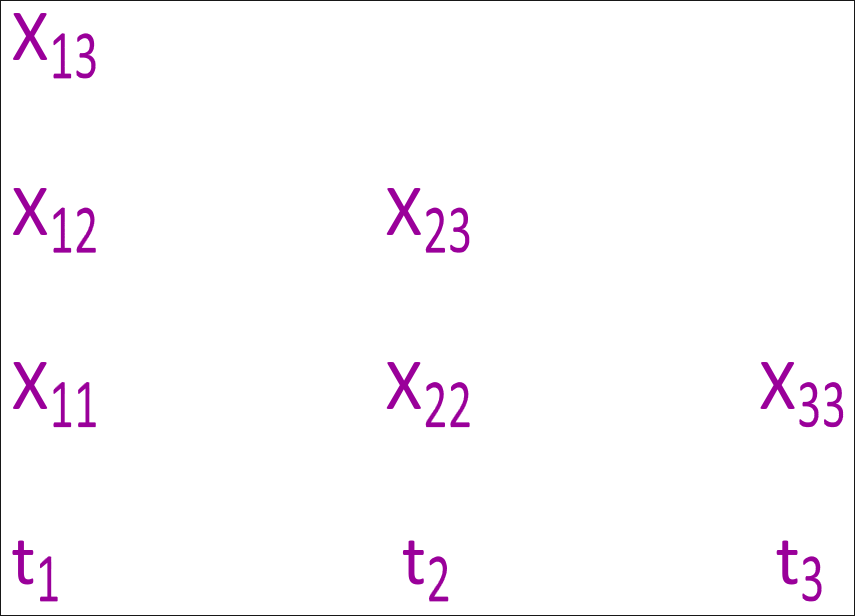
\includegraphics[width=.4\textwidth]{assets/20261119_165749.png}
    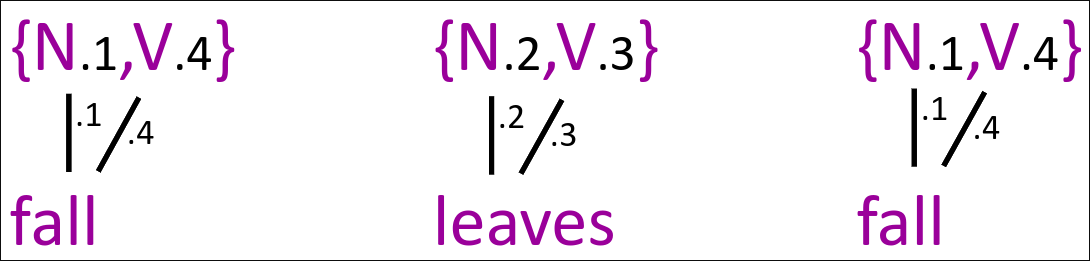
\includegraphics[width=.4\textwidth]{assets/20261119_165806.png}
    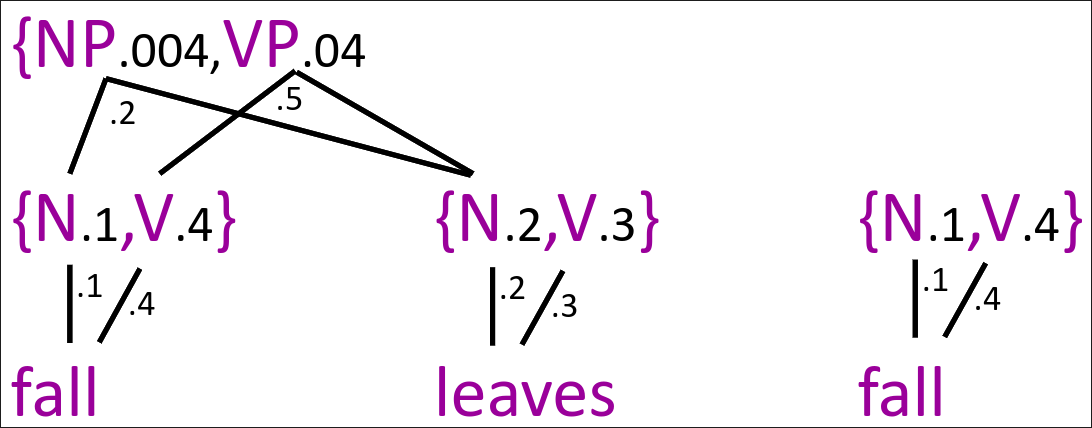
\includegraphics[width=.4\textwidth]{assets/20261119_165838.png}
    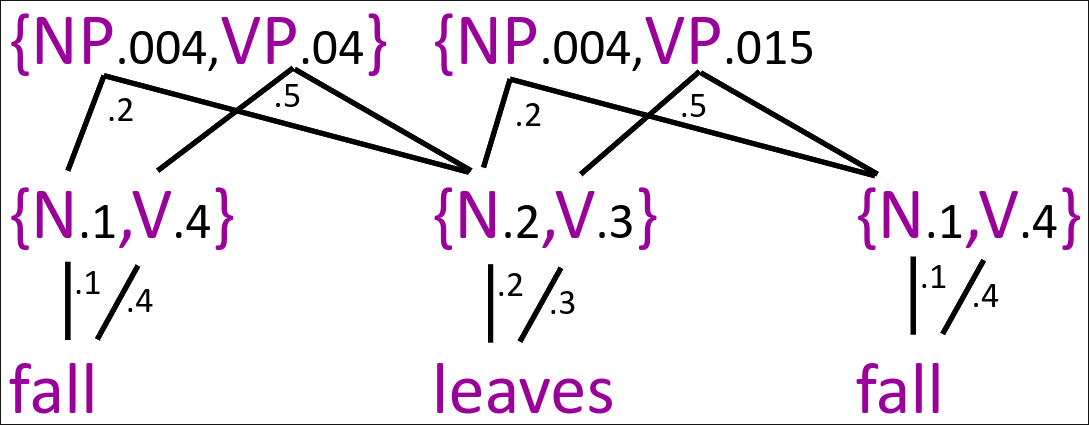
\includegraphics[width=.4\textwidth]{assets/20261119_165855.png}
    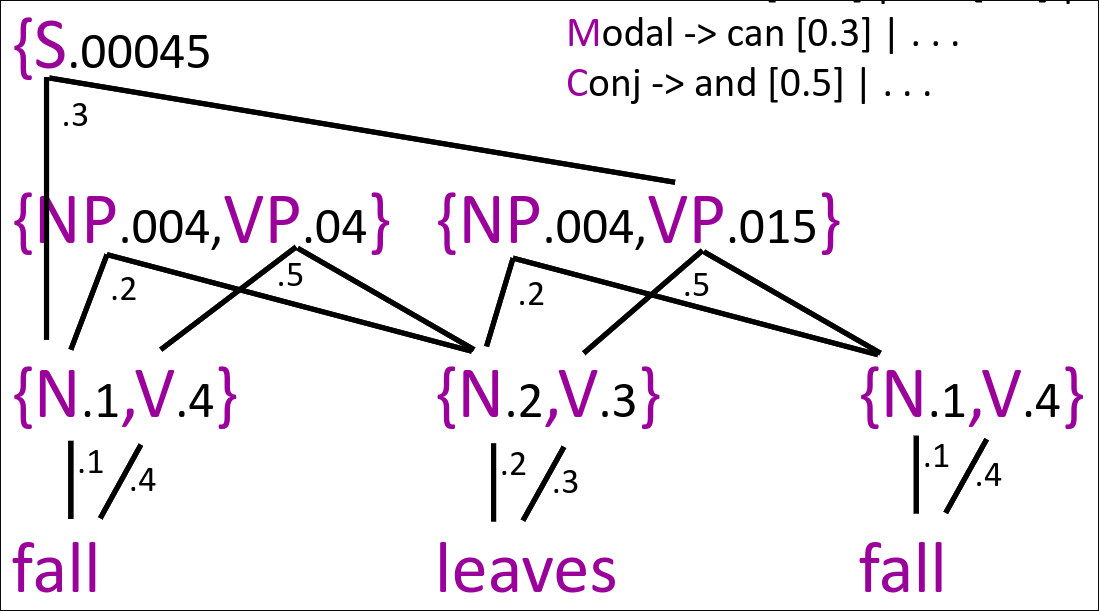
\includegraphics[width=.4\textwidth]{assets/20261119_170236.png}
    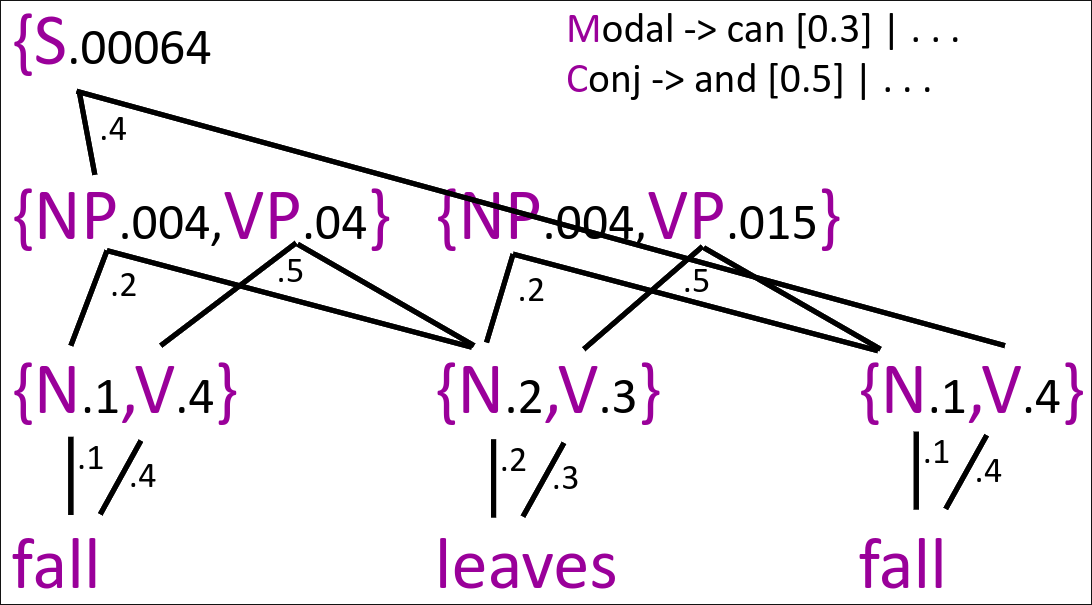
\includegraphics[width=.4\textwidth]{assets/20261119_170255.png}
    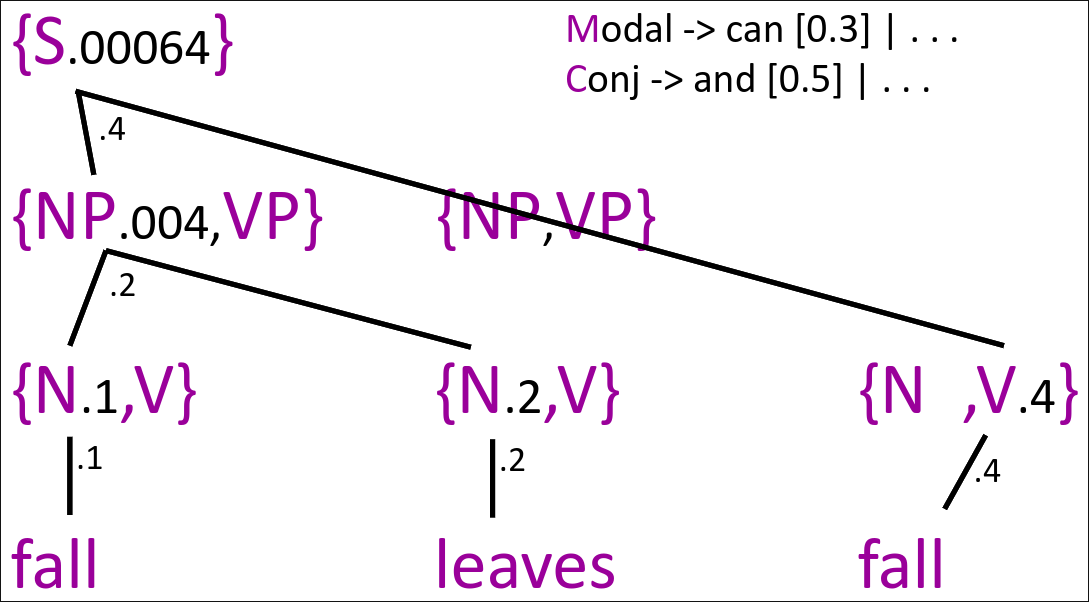
\includegraphics[width=.4\textwidth]{assets/20261119_170440.png}
\end{cimage}
Each variable $A\in X_{ij}$ is associated with the probability:
\[
    \max_{T\in Tree_G(\vc{t_i}{t_j}):root(T) = A}P_G(T)
\]
\begin{note}
    We just \textbf{keep backpointers} to \textbf{the variable pair} that generates the tree having the \textbf{maximum probability}
\end{note}
% subsubsection PCYK Algorithm (end)
%
\subsubsection{Inside Algorithm}\label{sub:in_inside_algorithm} % (fold)
The \textbf{Inside algorithm} performs the \textbf{observed string probability} inference task.
Again, a \textbf{probabilistic} variant of the \hyperref[sub:ll_algoritmo_cyk]{CYK Algorithm}, where \textbf{backpointers are not needed}, which efficiently infers the probability:
\[
    P_G(w) = \sum_{T\in Tree_G(w)}{P_G(T)}
\]
\begin{note}
    Same computational complexity as CYK: $O(n^3)$ with $n = |w|$
\end{note}
\begin{cimage}
    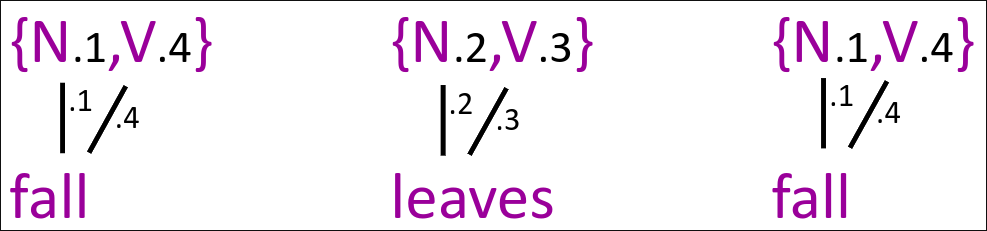
\includegraphics[width=.4\textwidth]{assets/20261119_173046.png}
    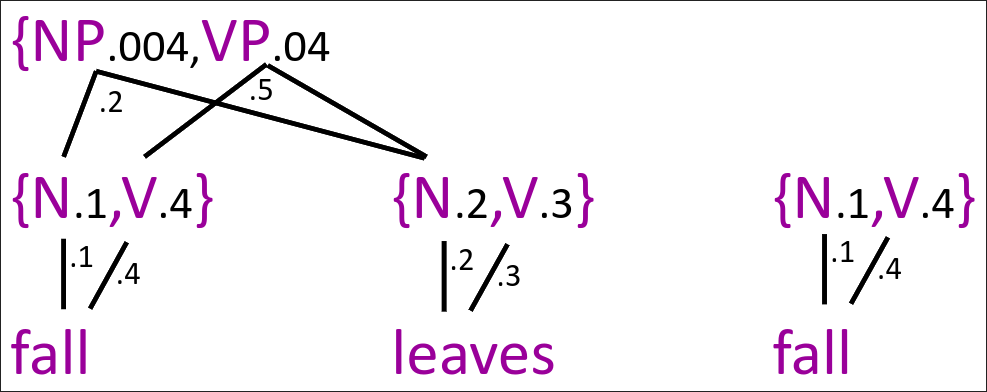
\includegraphics[width=.4\textwidth]{assets/20261119_173114.png}
    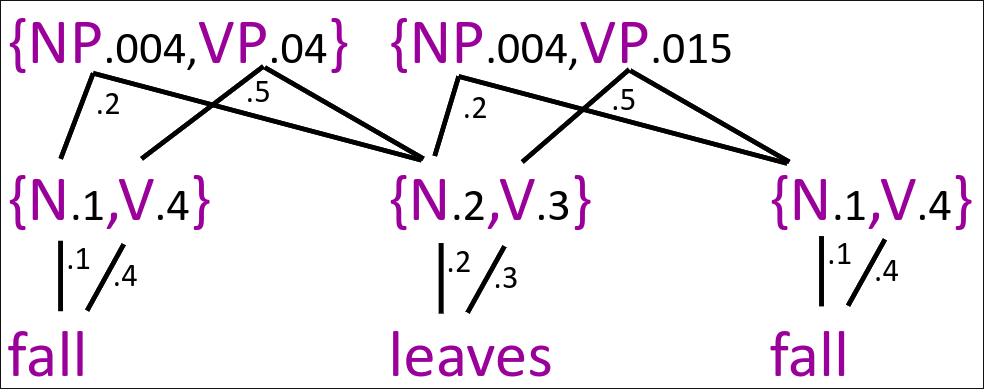
\includegraphics[width=.4\textwidth]{assets/20261119_173132.png}
    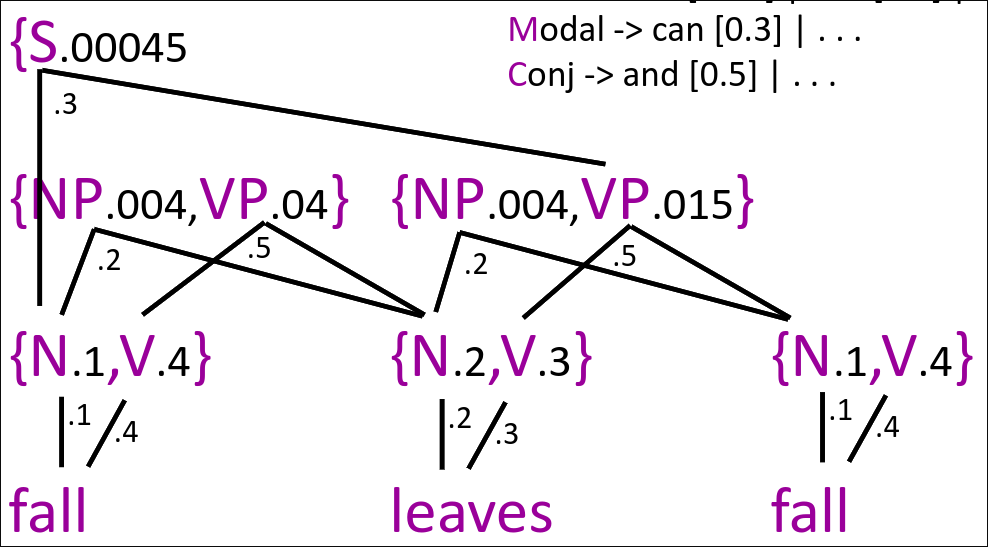
\includegraphics[width=.4\textwidth]{assets/20261119_173148.png}
    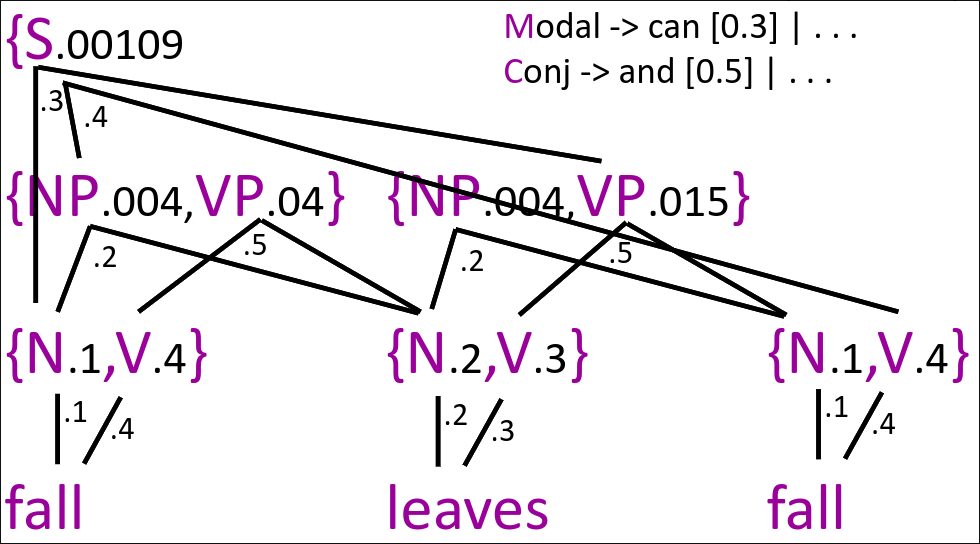
\includegraphics[width=.4\textwidth]{assets/20261119_173208.png}
    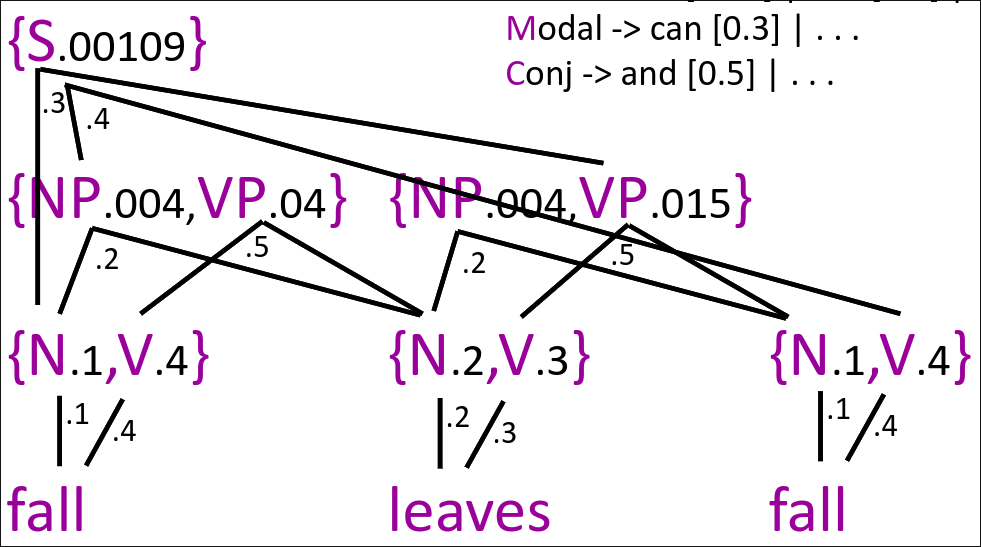
\includegraphics[width=.4\textwidth]{assets/20261119_173224.png}
\end{cimage}
Each variable $A\in X_{ij}$ is associated with the probability:
\[
    \sum_{T\in Tree_G(\vc{t_i}{t_j}):root(T) = A}P_G(T)
\]
% subsubsection Inside Algorithm (end)
% subsection PCFG Inference Algorithm (end)
% section PCFG Inference Task (end)
%
\section{Mixture of BOW Inference Task}\label{sec:in_mixture_of_bow_inference_task} % (fold)
\begin{description}
    \item[Maximum A Posteriori] It infers the $Categ'$ with \textbf{maximum} conditional probability:
        \[
            \ba[]{Categ'}{w} = \frac{\p{Categ',w}}{P(w)}
        \]
        As for \hyperref[def:pcfg]{PCFGs}, we can simply calculate:
        \[
            Categ' = \argmax_{Categ}{P(Categ,w)} = \argmax_{Categ}{\frac{P(Categ,w)}{p(w)}}
        \]
        \begin{note}
            Algorithmically, here the number of categories $Categ$ to consider is simply fixed
        \end{note}
\end{description}
%
\subsection{Bayes Theorem}\label{sub:in_bayes_theorem} % (fold)
Since $P(Categ,w) = \p{Categ}\ba[]{w}{Categ}$, the \textbf{Posterior probability distribution} can be written:
\[
    \ba[]{Categ}{w} = \frac{P(Categ)\ba[]{w}{Categ}}{P(w)}
\]
Thus, the \textbf{prior probability distribution} is $P(Categ)$: probability distribution over model \textbf{hidden structures} before the observation.
%
\subsubsection{Naive Bayes}\label{sub:in_naive_bayes} % (fold)
Moreover, since $\ba[]{w}{Categ} = \prod_{i = 1}^{N(w)}\ba[]{t_i}{Categ}$ with $N(w) = N+1,\,w = t_{1:N}$ and $T_{N+1} = \text{<EOS>}$, we have:
\[
    \ba[]{Categ}{w} = \frac{P(Categ)\prod_{i=1}^{N(w)}\ba[]{t_i}{Categ}}{P(w)}
\]
This specific form of the \hyperref[sub:in_bayes_theorem]{Bayes Theorem} is called \textbf{Naive Bayes}.
\emptyln{}
In general, consider $M$ data features:
\[
    \ba[]{Hypoth}{\vc{o_1}{o_M}} = \frac{P(Hypoth)\prod_{i=1}^{N(w)}\ba[]{o_i}{Categ}}{P(\vc{o_1}{o_M})}
\]
\begin{note}
    The term \textbf{Naive} comes from the fact that is based on an \textbf{independence assumption}: tokens $t_i$ with $1\le i\le N+1$ are \textbf{independently generated}
\end{note}
\begin{warning}
    \hyperref[sub:lm_mixture_of_bag_of_words]{Mixture of Bag-of-Words} generates \textbf{wrong English sentences}, but it is, anyway, good at \textbf{classifying a given sentence}
\end{warning}
\begin{definition}{Discriminative Model}{discriminative-model}
    Differently from \hyperref[def:generative-model]{Generative Models}, \textbf{discriminative models} are \textbf{specialized} in the \textbf{classification task}, evaluating its classification value/label; but a discriminative model cannot generate random words representative of a category
\end{definition}
% subsubsection Naive Bayes (end)
% subsection Bayes Theorem (end)
%
\subsection{Observation Sequence Generation}\label{sub:in_observation_sequence_generation} % (fold)
The \textbf{generation probability} of a string $w = o_{i:N}$, a sequence of observations $\vc{o_1}{o_N}$, via a state sequence $Seq = Categ_{1:N}$.
\begin{cimage}
    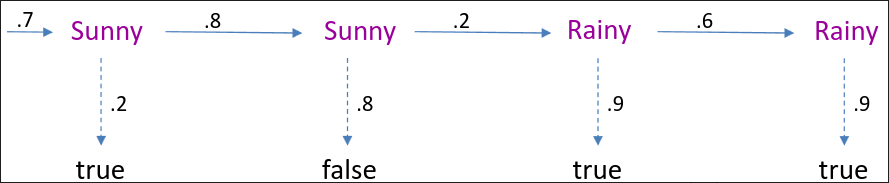
\includegraphics[width=.8\textwidth]{assets/20261120_114545.png}
\end{cimage}
With $w = \text{true false true true}$, $Seq = \text{Sunny} \to \text{Sunny}\to \text{Rainy}\to \text{Rainy}$:
\begin{ceq}
    P(Seq,w) = P(Seq)\ba[]{w}{Seq} = P(Seq)\prod_{i=1}^{N(w)}\ba[]{o_i}{Categ_i} = \\
    0.0672 \cdot 0.2 \cdot 0.2 \cdot 0.8 \cdot 0.9 \cdot 0.9 \\
    \text{where } P(Seq) = 0.7 \cdot 0.8 \cdot 0.2 \cdot 0.6 = 0.0672
\end{ceq}
\begin{example}{HMM and Terminating HMM Inference Tasks}{}
    Given \texttt{w = true false true false} generated via state sequences $Seq = \text{Sunny}\to \text{Sunny}\to \text{Rainy}\to \text{Rainy}$:
    \begin{ceq}
        P(Seq,w) = 0.00870912 \\
        P(w) = \sum_{Seq\in Seq(w)}P(Seq,w) \text{ with } |Seq(w)| = 2^4
    \end{ceq}
    \begin{description}
        \item[Maximum A Posteriori] It infers the state sequence $Seq'$ with \textbf{maximum} conditional probability:
            \[
                \ba[]{Seq'}{w} = \frac{P(Seq',w)}{P(w)}
            \]
            As for \hyperref[def:pcfg]{PCFGs} we can calculate:
            \[
                Seq' = \argmax_{Seq\in Seq(w)}{P(Seq,w)} = \argmax_{Seq\in Seq(w)}\frac{P(Seq,w)}{P(w)}
            \]
            we define $Seq(w)$ as the \textbf{set} of state sequences $Seq$ that can \textbf{generate} $w$, such that $|Seq| = N(w)$.
            \begin{note}
                For an \hyperref[def:hmm]{HMM} as $N(w) = |w|$, for a \hyperref[sub:lm_terminating_hidden_markov_models]{Terminating HMM} as $N(w) = |w| + 1$
            \end{note}
            In general, the \textbf{number} $|Seq(w)|$ of state sequences $Seq$ to consider is \textbf{exponential} in the length of $w$.
            \begin{tip}[Viterbi Algorithm]
            \end{tip}
        \item[Posterior Probability Distribution] It infers given any $Seq \in Seq(w)$:
            \[
                \ba[]{Seq}{w} = \frac{P(Seq,w)}{P(w)}
            \]
            In general $P(w) = \sum_{Seq\in Seq(w)}P(Seq,w)$ is computed by the \textbf{observed string probability inference} task: the number $|Seq(w)|$ of state sequences $Seq$ to consider is \textbf{exponential} in the length of $w$.
            \begin{tip}[Forward Algorithm]
            \end{tip}
    \end{description}
    In some tasks \textbf{posterior probability distribution} may be \textbf{marginalized} by focusing on some component of sequences $Seq$ that can generate $w$.
    \begin{example}{Filtering Focuses on the Last State}{}
        It infers the \textbf{posterior probability distribution} over the last state $last(Seq)$ of sequences $Seq\in Seq(w)$:
        \[
            \ba[]{Categ}{w} = \frac{P(w,Categ) = \sum_{Seq\in Seq(w):last(Seq) = Categ}P(Seq,w)}{P(w)}
        \]
        Again, the number of state sequences $Seq$ to consider is \textbf{exponential} in the length of $w$.
        \begin{note}[Actually]
            Filtering can be done during inference on $w$, \textbf{inductively} over prefixes of the $N(w)$ observations using a \textbf{polynomial variant} of the \textbf{Forward Algorithm}.
        \end{note}
    \end{example}
\end{example}
% subsection Observation Sequence Generation (end)
% section Mixture of BOW Inference Task (end)
%
\section{HMM Inference Algorithm}\label{sec:in_hmm_inference_algorithm} % (fold)
We use the Sunny/Rain \hyperref[def:hmm]{HMM} to exemplify \textbf{Viterbi} and \textbf{Forward} inference algorithm.
\emptyln{}
We start from the \textbf{Viterbi Algorithm} that performs the \textbf{Maximum A Posteriori} inference task.
Similar to the \hyperref[sub:in_pcyk_algorithm]{PCYK Algorithm} for \hyperref[def:pcfg]{PCFGs}, it \textbf{efficiently} infers the \textbf{state sequence} $Seq'$ such that the probability of \textbf{generating} $w$ via $Seq'$ is maximum:
\[
    Seq' = \argmax_{Seq\in Seq(w)}P(Seq,w)
\]
\begin{tip}[Computational Complexity: $O(n)$ with $n = |w|$]
\end{tip}
% section HMM Inference Algorithm (end)
% chapter Inference Tasks (end)
